% Requires graphicx; use figure, not figure*, for a single RevTeX column.
\begin{figure}[t]
  \centering
  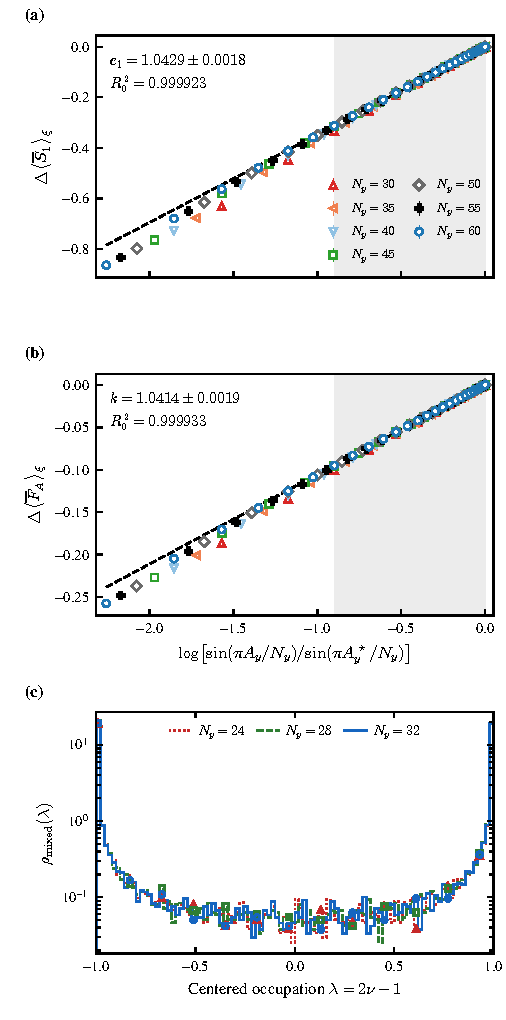
\includegraphics[width=\columnwidth]{endpoint_entropy_charge_spectrum_3x1.pdf}
  \caption{\textbf{Entropy, charge fluctuations, and half-system occupations.}
  Hard-wall circuits at $N_x=20$, starting from pure half-filled random states
  and evolved for $2N_y$ cycles, with $100$ independent trajectories per size.
  (a,b) Trajectory-averaged von Neumann entropy and intrinsic charge variance
  for $N_y=30,35,\ldots,60$. Periodic origins are averaged within each trajectory
  before averaging trajectories. Curves are anchored at
  $A_y^\star=\lfloor N_y/2\rfloor$; points at $A_y=1$ are omitted.
  Dashed lines are equal-size-weighted,
  through-origin fits over $A_y=8,\ldots,A_y^\star$, yielding $c_1=3m_S$
  and $k=\pi^2m_F$; shading spans the combined fit domain.
  Bars denote ordinary trajectory SEMs, and coefficient errors retain the
  covariance across strip widths.
  (c) Centered half-system occupations $\lambda=2\nu-1$ from a separate
  ensemble at $N_y=24,28,32$, for $[0,20)\times[0,N_y/2)$.
  Eigenvalues are pooled over trajectories, retaining
  $|\lambda|<1-10^{-8}$; each density has unit area over the retained modes.
  The vertical axis is logarithmic.}
  \label{fig:entropy-charge-spectrum}
\end{figure}
